\documentclass{standalone}

\usepackage[utf8]{inputenc}
\usepackage{tikz,fp,siunitx}
\usetikzlibrary{decorations.pathreplacing}

\begin{document}
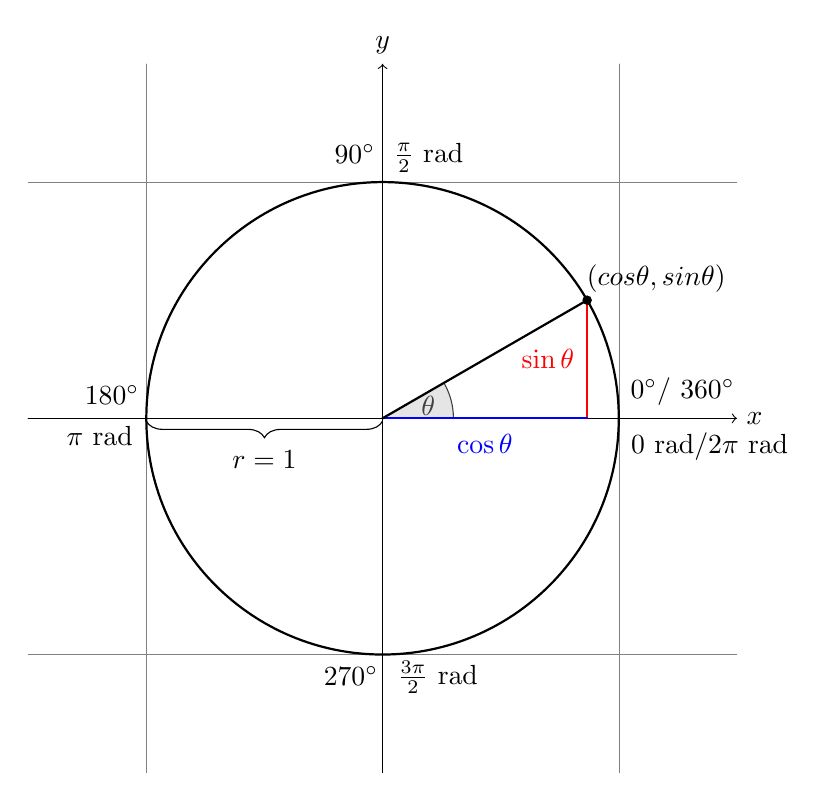
\begin{tikzpicture}[scale=3,cap=round]

    % Draw background grid
    \draw[style=help lines,step=1cm] (-1.5,-1.5) grid (1.5,1.5);

     % Axes
    \draw[->] (-1.5,0) -- (1.5,0) node[right] {$x$};
    \draw[->] (0,-1.5) -- (0,1.5) node[above] {$y$};

    % Draw the circle itself
    \draw[thick] (0,0) circle (1);

    \draw[decorate,decoration={brace,amplitude=6pt,raise=1pt},yshift=0pt] (0,0) -- (180:1) node [midway,xshift=0,yshift=-15pt] { $r = 1$ };

    % Label 0 deg
    \node at (5:1.275) {\ang{0}/ \ang{360}};
    \node at (-5:1.39) {0 rad/$2\pi$ rad};

    % Label 90 deg
    \node at (96:1.125) {\ang{90}};
    \node at (80:1.12) {$\frac{\pi}{2}$ rad};

    % Label 180 deg
    \node at (175:1.15) {\ang{180}};
    \node at (183.5:1.2) {$\pi$ rad};

    % Label 270 deg
    \node at (263:1.1) {\ang{270}};
    \node at (282:1.12) {$\frac{3\pi}{2}$ rad};


    \colorlet{anglecolor}{gray!50!black}
    \colorlet{sincolor}{red}
    \colorlet{coscolor}{blue}
    % cos 30 in rad
    \def\cosThirty{0.8660256}
    
    
    \filldraw[fill=gray!20,draw=anglecolor] (0,0) -- (3mm,0pt) arc(0:30:3mm);
    \draw (15:2mm) node[anglecolor] {$\theta$};
    
    \draw[thick,sincolor] (30:1cm) -- node[left=1pt] {$\sin \theta$} ++(0,-.5);

    \draw[thick,coscolor] (0,0) -- node[below=2pt] {$\cos \theta{}$} (\cosThirty,0);
    
    \draw[thick] (0,0) -- (30:1);
    
    \node at (27:1.3) {$(cos \theta, sin \theta)$};
    \draw plot [mark=*, mark size=0.5] coordinates{(30:1)}; 

\end{tikzpicture}

\end{document}
